\documentclass[14pt,oneside]{extreport}

% Font
\usepackage[T1]{fontenc}
\usepackage[utf8]{inputenc}
\usepackage{lmodern}

% For tables
\usepackage{adjustbox}
\usepackage{multirow}

% For identing the table at the right place
\usepackage{float}

% For images
\usepackage{graphicx}
\usepackage[labelfont=bf]{caption}
\graphicspath{ {./images/} }

% links
\usepackage{hyperref}

% items spacing
\usepackage{enumitem}

% for shorter paragraph spaces
\setlength{\parindent}{1ex}
\setlength{\parskip}{0.5ex}
% for first paragraphs
\newcommand*\fpar{\hspace{1ex}}

\title{\textbf{Cloud Storage Systems} \\
       \large Project - Phase 10 Essay}
\date{\textbf{Group 14} \\ 25/05/2021}
\author{
Tiago Carvalho    \\
\texttt{fc51034}  \and
Diogo Lopes       \\
\texttt{fc51058}  \and
Miguel Saldanha F  \\
\texttt{fc51072}  \and
João Roque        \\ 
\texttt{fc51080}  \and
João Afonso       \\ 
\texttt{fc51111}
}

% Essay:
% - font size 14
% - Arial, Verdana, Calibri, Universe, Helvetica, ...
% - Single Column
% - Headings for main sections, one or two levels
% Topics:
%   - Abstract
%   - Papers 1-5
%       - 2 to 3 pages per paper
%   - Conclusion

\begin{document}
\maketitle

\begin{abstract}
  \fpar Cloud Storage is a really complex field, and systems implementing it are growing, both in terms of complexity and scalability. Providing faster service to more and more users. 
  \par But everything comes at a cost, and cloud storage systems cannot have everything we wish for, like Consistency, Availability and Partition Tolerance, that is called CAP Theorem, and we must pick a ratio of them. Thankfully there are already a lot of different models and methods to attenuate this problem.
  \par TODO
\end{abstract}

% Chapter 1 - João Roque
\chapter{\Large{A brief survey on replica consistency in cloud environments \cite{paper1}}}
  \section{State of the art}
  \fpar Databases are, very usually, the core of a cloud service, either for enterprises or actual costumers. With increasing importance it's expected to perform for its users.
  \par A database is expected to be Consistent, where the latest read expects the most recent write; Available, where every read should receive a valid response (instead of an error); and Partition tolerant, meaning it's expected that the system keeps working even if something fails, like a database node, network problems, etc...
  \par And this can be possible on a single database, even assuring the ACID properties, however, on a cloud database there's synchronization that needs to take place to achieve consistency, and everything comes at a cost, and that's what the CAP theorem states: It is impossible for a distributed data storage to, simultaneously, provide more than two of the three properties stated before (Consistency, Availability, and Partition Tolerance).
  \par Cloud services try to maintain the balance between these 3 properties. If it is important to have consistency, maybe decreasing the response time, availability, helps with that, spreading changes to other partitions, or maybe the partitions are not the most important aspect, and then its amount is reduced, meaning there are fewer partitions to update and synchronize, increasing once again the availability.
  \par There are many example of usage, and there's always a sacrifice in either one of the three properties to improve on the others, as we will show in this chapter.

  \section{Consistency}
    \subsection{Data/Client-centric consistency models}
    \fpar Between the data center and the clients there's already a choice to be made, if the client should be a part of keeping the data consistent, or not.
    \par Each option, obviously, has its own pros and cons. For the Data-centric these are the general options, in order of consistency provided:
    \begin{itemize}[noitemsep]
      \item \textbf{Week} - There is no “supervision”, the first item found is returned.
      \item \textbf{FIFO} - There are no guarantees besides writes from the same process being synchronized, using a First In First Out approach.
      \item \textbf{Causal} - Consistency is only guaranteed between requests with a causal dependency.
      \item \textbf{Sequential} - All operations are serialized in the same order in all partitions, and every operation keeps its received internal order.
      \item \textbf{Strict} - For each received write it needs to be instantaneously spread to other partitions to be updated.
    \end{itemize}
    \par And then for the Client aspect:
    \begin{itemize}[noitemsep]
      \item \textbf{Eventual} - All updates will eventually propagate far enough that every partition gets updated.
      \item \textbf{Monotonic read} - Guarantees that for each read the result will never be older than the same reads before.
      \item \textbf{Monotonic write} - Different writes from the same request are always processed in the same order.
      \item \textbf{Read-your-writes} - Guarantees, for the same request, that for each write the next read will never return an older result than that write.
      \item \textbf{Writes-follow-reads} - For the same request, each write after a read, guarantees that will be executed on the same or more recent value of the previous read.
    \end{itemize}

    \subsection{Replica consistency methods}
    \fpar As stated a cloud database can have many partitions, and if we are replicating the data it needs to be identical, so any access doesn't get wrong results. These are the methods that are usually applied:
      \subsubsection{Fixed consistency methods}
      \begin{itemize}[noitemsep]
        \item \textbf{Event sequencing-based}, simple method that hides replication complexity, focusing on availability.
        \item \textbf{Clock-based strict}, relies on timestamps and avoids concurrent accesses.
      \end{itemize} 
      \subsubsection{Configurable consistency methods}
      \begin{itemize}[noitemsep]
        \item \textbf{Automated and self-adaptive}, enforces multiple levels of consistency over distinct data.
        \item \textbf{Flexible}, can have distinct approaches that dynamically change their consistency ratio.
      \end{itemize} 
      \subsubsection{Consistency monitoring methods}
      \begin{itemize}[noitemsep]
        \item \textbf{Consistency verification}, to verify and detect possible protocol or contract violations by the cloud service.
        \item \textbf{Consistency auditing}, a large data cloud and multiple small audit clouds with groups of users that cooperate on a specific job. They share a service-level agreement and the audit cloud verifies if it's violated.
      \end{itemize} 

% Chapter 2 -Diogo Lopes
\chapter{\Large{Autoscaling tiered cloud storage in Anna \cite{paper2}}}
  \section{Motivation}
  \fpar A wide variety of cloud-storage systems is available nowadays, and developers can select the one that better suits their application’s needs, making cost-performance trade-offs. However, these systems are not very dynamic, which is not ideal when most applications deal with a non-uniform distribution of performance requirements.

  \section{Overview of Anna}
  \fpar Anna is an autoscaling, multi-tier, coordination-free, distributed key-value store service for the cloud that allows system operators to specify service-level objectives (SLOs), like fault tolerance or cost-performance. It is built on AWS components.
  \par The performance of a system depends on the volume of a workload and on whether workloads make a lot of requests to a small subset of the keys or more uniform requests. Anna uses three mechanisms to adapt to these dynamics of workloads:
  \begin{itemize}[noitemsep]
    \item \textbf{Horizontal elasticity} – Storage tiers can increase/decrease storage capacity and compute and networking capabilities, depending on the volume of a workload, by adding/removing nodes.
    \item \textbf{Multi-Master Selective Replication} – Hot sets (frequently accessed) are replicated onto many machines, with hot keys being more replicated than cold ones.
    \item \textbf{Vertical Tiering} – Anna is able to promote hot data to the fast, memory-speed tier and demote cold data to cold storage.
  \end{itemize}

  \section{Anna Architecture}
  
  \begin{figure}[htbp]
    \centerline{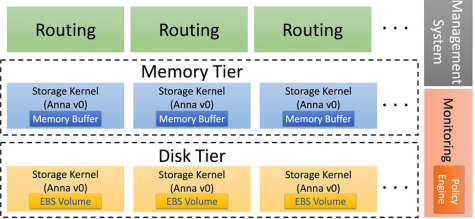
\includegraphics[scale=0.5]{images/paper2/architecture.png}}
    \caption{Anna architecture.}
    \label{fig}
  \end{figure}

  \begin{figure}[htbp]
    \centerline{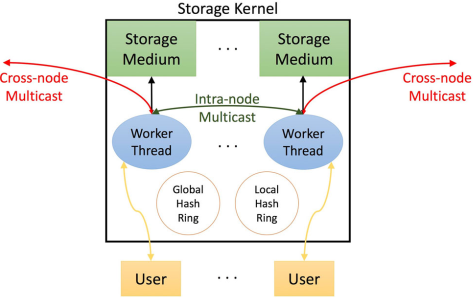
\includegraphics[scale=0.5]{images/paper2/storage_kernel.png}}
    \caption{The architecture of storage kernel.}
    \label{fig}
  \end{figure}

  \begin{figure}[htbp]
    \centerline{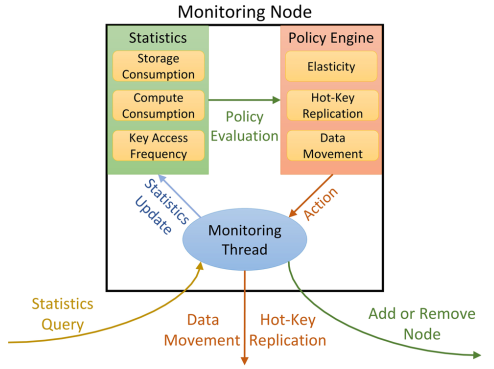
\includegraphics[scale=0.5]{images/paper2/monitoring_node.png}}
    \caption{The architecture of a monitoring node.}
    \label{fig}
  \end{figure}

  \fpar Anna has two storage tiers: one that is fast but expensive, providing RAM cost-performance, and another that is slow but cheap, providing flash disk cost-performance.
  \par The \textbf{monitoring system} and \textbf{policy engine} are responsible for adjusting the system to the workloads’ dynamics and meet the SLOs. The \textbf{cluster management system} modifies resource allocation based on the decision of the policy engine (with Kubernetes). \textbf{Routing service} is an API that abstracts the internal dynamics of the system.
  \par Each \textbf{storage kernel} contains multiple threads that interact with a thread-local storage medium (memory-buffer or disk volume, depending on the tier) and process requests from clients.
  \par Shared-memory coordination and consensus algorithms decrease performance and cause latency and availability issues. Therefore, Anna is coordination-free. Periodically, threads multicast (gossip) updates to others that have replicas of their keys. Conflicts are resolved asynchronously. As a result, Anna exploits multi-core parallelism within a single machine and smoothly scales out across distributed nodes.
  \par For different key replicas, although a set of gossips may be applied in different orders, \textbf{Commutativity}, \textbf{Associativity}, and \textbf{Idempotence} properties ensure that the state of the replicas eventually converges.
  \par Anna uses metadata to efficiently support the mechanisms initially described. Each tier has two \textbf{hash rings}. A global one that determines which nodes are responsible for storing each key and a local one that determines the set of threads within a node that are responsible for a key. Each key has a \textbf{replication vector} that has the number of nodes in each tier, and the number of threads per node in each tier storing it. Anna also tracks \textbf{monitoring statistics}, like the access frequency of each key and the storage consumption of each node.

  \section{Policy Engine}
  \fpar Anna supports three kinds of SLOs: an \textbf{average request latency} (ms), a \textbf{cost budget} (dollars/h), and a \textbf{fault tolerance} (number of replicas that are allowed to fail). If the average storage consumption in a tier has violated configurable upper/lower thresholds, nodes are added/removed. Then data is promoted or demoted across tiers. Next, if the latency exceeds a certain fraction of the latency SLO and memory tier’s compute consumption exceeds a threshold, nodes are added to the memory tier. However, if not all nodes are occupied, hot keys are replicated in the memory tier. Finally, if the observed latency is a certain fraction below the SLO and the compute occupancy is below a threshold, the system checks if it can remove nodes to save cost.

  \section{Anna API}
  
  \begin{figure}[htbp]
    \centerline{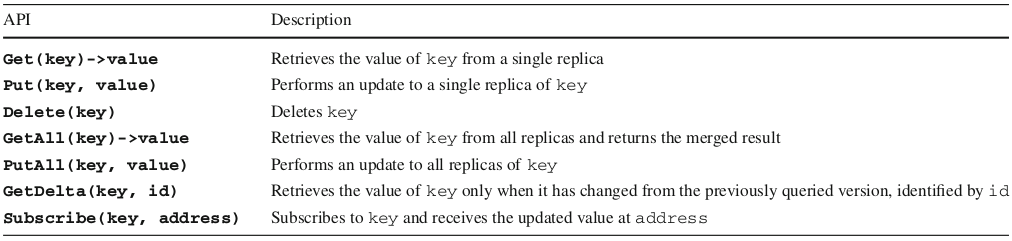
\includegraphics[scale=0.5]{images/paper2/API.png}}
    \caption{Anna API.}
    \label{fig}
  \end{figure}

  \fpar GetAll allows users to observe the most up-to-date state of a key. Put relies on asynchronous gossip for the update to propagate to other replicas. If the node crashes before gossiping, the update will be lost.

  \section{Conclusion}
  \fpar Integrating the mechanisms described, Anna becomes an efficient, autoscaling system representing a new design point for cloud storage. In many cases, Anna is orders of magnitude more cost-effective than popular cloud storage services and prior research systems. Throughput increases linearly with cost, meaning that it can get better performance out of the same cost when compared to available cloud storage solutions. Also, the system is able to adapt to dynamic workloads while not violating the SLOs most of the time. Finally, the system is able to recover from node crashes, while not hurting performance too much, since it does not pause, providing high availability to the users.

% Chapter 3 - Miguel Saldanha
\chapter{\Large{Threats and security issues in cloud storage and content delivery networks: Analysis \cite{paper3}}}
In this paper is adressed the security threaths to Cloud Storage and one of it´s uses as Content Delivery Network.
\section{Issues and challenges of CS and CDN}
\fpar
\section{Threath model of CS used as CDN}
\fpar
\begin{figure}
    \centering{
    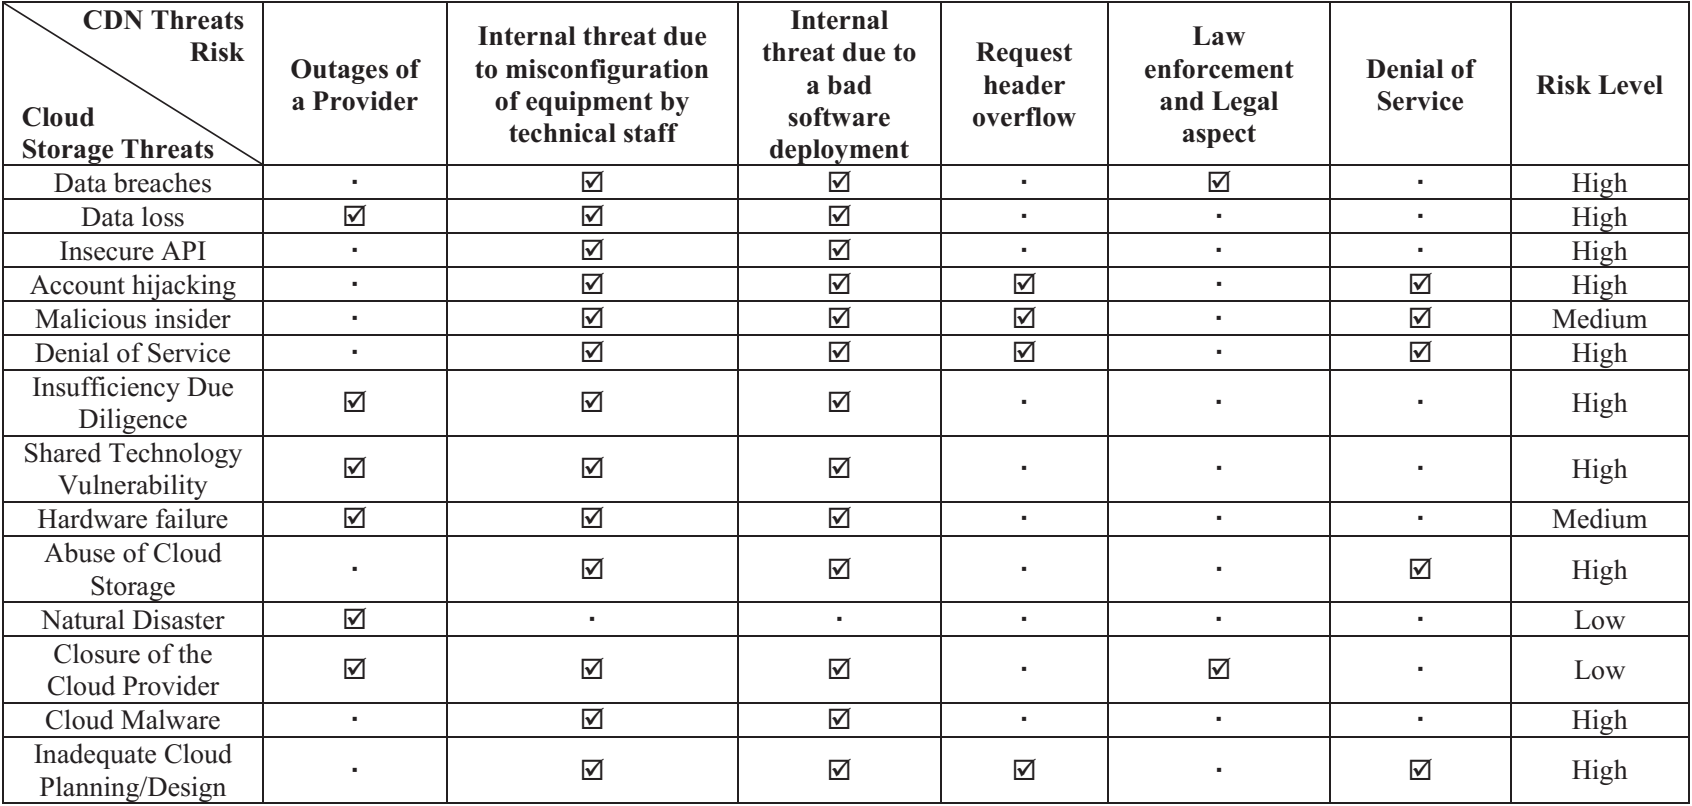
\includegraphics[scale=0.25]{./images/paper3/3_table.png}}
    \caption{Matrix of common content delivery network threats in cloud storage used as content delivery network}
    \label{fig:2}
\end{figure}

\section{Threath model of CS used as CDN}

% Chapter 4 -Tiago Carvalho
\chapter{\Large{Data auditing in cloud storage using Smart Contract \cite{paper4}}}
\fpar With any distributed storage system, such as cloud storage, there are many issues that one needs to be aware of: consistency, fault tolerance and integrity, to name a few. This paper focus especially on the integrity problem. Despite cloud storage systems using the usual mechanisms to avoid data corruption, like RAIDs and ECCs, there are still problems that arise, and usually it is needed to resort to a Third Party Auditor (TPA). This TPA is responsible to check for the integrity of the data to reassure that nothing has been corrupted. While this works, there are privacy, security and confidentiality concerns when using a TPA since they have access to all the data and things can be compromised. To address this problem, the authors propose the usage of smart contracts to perform this data auditing.
\section{Smart Contracts in Data Auditing}
To put it simply, a smart contract is a piece of code that is deployed on a blockchain for the participating nodes to execute in exchange for gas. Since a blockchain is a fully decentralized system, it avoids entirely the chance of a third party tampering with the data, since the blockchain technology on itself is specialized with dealing with this kind of problems.
\subsection{Proposed System}
To implement it, the researchers proposed an architecture which comprises three elements: the Cloud Service Provider (CSP), the Data Owner and a blockchain. The blockchain used was Ethereum-based since it is the more popular blockchain to support smart contracts. In this architecture, the user sends the data encrypted to the CSP, hashing it beforehand. This hash is then used in the creation of the smart contract, by the user. The smart contract includes information about the data such as the name of the files, hashes, size and details of the data own, as well as other relevant info. This smart contract is then deployed on the blockchain to perform the data auditing periodically. One thing worth noting is that the researchers used an optimized blockchain for data auditing, the DAB (Data Auditing Blockchain), designed for this sole purpose.
\subsection{Performance Analysis}
After the system was designed and implemented, the authors did an evaluation on its performance, with very positive results. They stated that the system provided reliable and confidential auditing, without requiring any effort from the CSP or user after the smart contract is deployed. The gas costs increased in a linear fashion depending on the number of blocks which is positive.
\section{Conclusion}
In this paper, the researchers presented the problem of data auditing in cloud storage systems and gave a valid solution to it, the usage of smart contracts for data auditing. Its implementation is relatively simple, while having very good results, which is definitely a step in the right direction and could see further developments in the future. While the results achieved by the researchers were good, there are probably optimizations that can be done when developing the system for a real world use.

% Chapter 5 - João Afonso
\chapter{\Large{Key challenges and research direction in cloud storage \cite{paper5}}}
\fpar This paper provides a general overview of the issues, challenges and future trends associated with cloud storage and compares the approaches that are being taken by researchers to deal with these problems.

\section{Issues in cloud storage}
\begin{itemize}[noitemsep]

\item \textbf{Data management:} The management of data stored across multiple geo-distributed data centers is associated with certain challenges: scalability, parallelism, recovery, consistency in replication, reliability, and cost.

\item \textbf{Data partitioning:} Partitioning is meant to improve scalability, optimizes performance, and reduce contention. There are two major types of partitioning techniques: horizontal and vertical partitioning. If fragmented data is distributed throughout all servers to take server capacity into account, then it is possible to achieve load balancing. Partitioning is supposed to solve the following problems: speed and availability.

\item \textbf{Data placement:} Has an important role in terms of performance in the cloud environment. Some main issues include: Geographically Distant Data Sharing, Client Mobility, Data Inter-dependencies.

\item \textbf{Availability through replication:} Process of sharing information to provide availability, reliability, fault-tolerance and accessibility and reduce response time / energy and bandwidth consumption. Data resources can be replicated closer to the application to reduce network latency. Challenges of replication: Data selection, Consistency in replicated data, sophisticated management, load balancing and recovery. Researchers have proposed solutions to minimize the replication cost and maximize the expected availability of objects.

\item \textbf{Data security:} Issues related to data security/theft, data unavailability, privacy, integrity.

\end{itemize}

\section{Open research challenges and future trends}

\begin{itemize}[noitemsep]

\item \textbf{Multicloud:} Prevents downtime, facilitates replication and fragmentation and improves security and costs. This approach adds complexity to application management (increased effort needed).

\item \textbf{DevOps in Cloud:} Bridges the gap between developers and operation team. DevOps tools can assist the management and configuration of resources (such as storage, networking, and computing). This approach improves both speed and productivity.

\item \textbf{Machine Learning in cloud:} Researchers are taking advantage of distributed environments to research parallelization of machine learning and data mining problems.

\item \textbf{Big Data in cloud:} There are still many challenges to overcome: scalability, availability, data integrity, data transformation, data quality, data heterogeneity, privacy, and legal issues.

\item \textbf{IOT in cloud and Fog Computing:} Enables new opportunities: complex analysis, data mining and real-time processing. Fog computing is an alternative to cloud computing that aims to bring the cloud closer to where data is created and acted upon.


\end{itemize}

\fpar To solve these challenges it is necessary to solve the following issues:
\begin{itemize}[noitemsep]
\item \textbf{Fragmentation:} Reducing data migration by providing workload aware dynamic fragmentation techniques.
\item \textbf{Data placement:} Providing a proper data placement strategy by considering factors like prediction of resource consumption and data locality.
\item \textbf{Data management:} Design of data management strategy with consideration of buffer management and memory cost.
\item \textbf{Replication:} Design an efficient and dynamic data replication strategy with consistency and fragmentation strategy. Designing an efficient data replication and consistent management strategy in geo distributed cloud by considering data pattern and network load factors.
\end{itemize}

\section{Conclusion}
\fpar Cloud storage still presents many problems that have yet to be solved. As such, researchers have been taking into consideration factors like: optimizing monetary cost, reducing network latency, optimal storage, increasing performance or optimal resource utilization (among others). It is also important to take into consideration that the way in which these problems are addressed will depend on the characteristics of the application in question.

\bibliographystyle{unsrt}
\bibliography{essay}

\end{document}